\documentclass[a4paper, 12pt]{report}
\usepackage[ngerman]{babel}
\usepackage{amssymb}
\usepackage[utf8]{inputenc}
\usepackage{amsmath}
\usepackage{bbm}
\usepackage{setspace}
\usepackage{graphicx}
\usepackage[style=alphabetic ,backend=biber]{biblatex}
\usepackage{csquotes}
\usepackage{geometry}
\geometry{
 a4paper,
 total={170mm,257mm},
 left=25mm,
 right=40mm,
 top=25mm,
 bottom=40mm
 }
 \setstretch{1.5}
\addbibresource{../Facharbeit/literatur.bib}
\usepackage{listings}
\usepackage{xcolor}

\definecolor{codegreen}{rgb}{0,0.6,0}
\definecolor{codegray}{rgb}{0.5,0.5,0.5}
\definecolor{codepurple}{rgb}{0.58,0,0.82}
\definecolor{backcolour}{rgb}{255,255,255}

\lstdefinestyle{codehighligthing}{
    backgroundcolor=\color{backcolour},
    commentstyle=\color{codegreen},
    keywordstyle=\color{magenta},
    numberstyle=\tiny\color{codegray},
    stringstyle=\color{codepurple},
    basicstyle=\ttfamily\footnotesize,
    breakatwhitespace=false,
    breaklines=true,
    captionpos=b,
    keepspaces=true,
    numbers=left,
    numbersep=5pt,
    showspaces=false,
    showstringspaces=false,
    showtabs=false,
    tabsize=2
}
\lstset{style=codehighligthing}

\title{Facharbeit Informatik}
\author{Joel Mantik}
\begin{document}
\maketitle
\begin{sloppypar}
\tableofcontents

\chapter{Einleitung}
\begin{quote}
    "The simplest model in applied mathematics is a system of linear equations. It is also by far the most important."
    \newline GILBERT STRANG
\end{quote}
Der Gauß-Algorithmus ist eins der wichtigsten Lösungsverfahren zum Lösen linearer Gleichungssysteme.
Er spielt eine tragende Rolle in vielen Bereichen der Mathematik und ist dennoch  recht unkompliziert.
    Aufgrund der Wichtigkeit, habe ich dazu entschieden, den Algorithmus in dieser
Facharbeit zu implementieren,
zu analysieren, und Anwendungsmöglichkeiten aufzuzeigen.

\chapter{Theoretische Grundlagen}
Der Gauß-Algorithmus ist ein Algorithmus, welcher beim Lösen von linearen Gleichungssystemen zum Einsatz kommt. Im folgenden Kapitel wird die mathematische
Theorie erläutert und die Definitionen genannt, welche die Grundlage für die spätere Implementierung sind.

\section{Lineare Gleichungssysteme}
Ein lineares Gleichungssystem ist eine Sammlung von Gleichungen, in denen jede Unbekannte mit höchstens dem ersten Grad vorkommt.
Es kann in der Form $ A_x = b $ geschrieben werden, wobei $A$ eine $ m x n $ Matrix ist, $x$ ein n-dimensionaler Vektor von Unbekannten
und b ein $m$-dimensionaler Vektor von Konstanten ist.
Ein allgemeines lineares Gleichungssystem lässt sich wie folgt definieren.:\cite{1}
\begin{align}
\label{eq:linGle}
    a_{11}x_{1}+ a_{12}x_{2}+\hdots+ a_{1n}x_{n} &=& b_1 \nonumber \\
    a_{21}x_{1}+ a_{22}x_{2}+\hdots+ a_{2n}x_{n} &=& b_2 \nonumber\\
                                                 &\vdots&  \nonumber \\
    a_{m1}x_{1}+ a_{m2}x_2+\hdots+a_{mn}x_{n} &=& b_{m}
\end{align}
Das Ziel eines solchen linearen Gleichungssystems ist es, eine Lösung für $x$ zu finden, die alle Gleichungen erfüllt.
Hierbei gibt es drei Arten von Lösungen:
\begin{enumerate}
    \item Das Gleichungssystem hat genau \textit{eine} Lösung; es gibt genau eine Lösung, welche alle Gleichungen im System
        erfüllt. Die Lösungsmenge ist z. B. : $\mathbb{L} = \{ (x,y,z)| (1,2,3)\} $.
    \item Das Gleichungssystem hat \textit{keine} Lösung, wenn es keine Lösung gibt,
        die alle Gleichungen erfüllt. Die Lösungsmenge ist eine leere Menge: $ \mathbb{L}= \emptyset$.
    \item Das Gleichungssystem hat \textit{unendlich viele} Lösungen, wenn es mehrere Lösungen gibt
        die alle Gleichungen im System erfüllen.
        Hierbei sind die verschiedenen Variablen voneinander abhängig.
        Die Lösungsmenge sieht beispielsweise wie folgt aus: \newline $ \mathbb{L} = \{(x, y, z)| (x = ay + z, y\in \mathbb{R}, z \in \mathbb{R}) \} $.
\end{enumerate}


\section{Gaußsches Eliminationsverfahren} \label{2.2}
\newline
Gegeben sei das Allgemeine Lineare Gleichungssystem \ref{eq:linGle}. Gesucht ist nun die Menge der $ (x_1, \hdots ,x_n ) \in \mathbb{R}^n $, die alle Gleichungen erfüllen.
Dies erreicht man, indem man folgendermaßen vorgeht.:
\begin{enumerate}
    \item Die erweiterte Koeffizientenmatrix $ (A, b) $ aufschreiben. \cite{2}:
        \begin{equation}
            (A, b):=
            \begin{pmatrix}
                a_{11} & \hdots &  a_{1n} &  b_1  \\
                \vdots & \vdots &  \vdots & \vdots &  \\
                a_{m1} &  \hdots &  a_{mn} &  b_m \\
            \end{pmatrix}
        \end{equation}
    \item $A$ durch elementare Zeilentransformationen, also Vertauschen von Zeilen, Multiplikation einer Zeile mit einer Zahl $\neq 0 $ oder Addition des Vielfachen von einer Zeile zu einer anderen Zeile auf Zeilenstufenform bringen.
        Eine $ m x n $-Matrix A heißt in \textit{Zeilenstufenform}, wenn sie von der folgenden Form ist: \newline \newline
        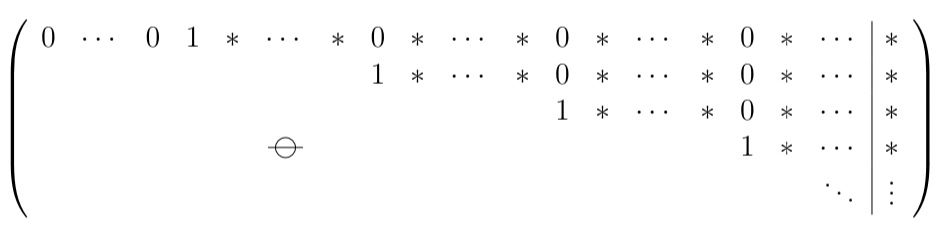
\includegraphics[width=350px]{"./Zeilenstufenform.jpeg"} \newline \newline
        Dabei steht der Stern für eine beliebige Zahl, und die freien Plätze sind alle mit Nullen besetzt. Der erste von Null verschiedene Eintrag in jeder Zeile ist 1. Dieser Eintrag wird das Pivot-Element der Zeile genannt.
        Das Pivot-Element der $(i + 1)$-ten Zeile steht immer rechts des Pivot-Elements der i-ten Zeile, und alle Einträge oberhalb eines Pivot-Elements sind gleich Null. \cite{5}
    \item Nun lassen sich durch Rücksubstitution die Werte für die Variablen ermitteln. Man teilt die letzte Spalte durch den Wert des Koeffizienten, so dass die Variable alleine steht.
          Der gefundene Wert wird dann in die nächst höhere Zeile eingesetzt, dann wird analog zum ersten Schritt vorgegangen.
\end{enumerate}

{\let\clearpage\relax \chapter{Implementierung des Algorithmus}}
Für die im Folgenden dargelegte Implementation und Analyse des Algorithmus wurde die Programmiersprache "Java" verwendet.

\section{Erläuterung des Quellcodes}
Der grundlegende Aufbau des Programms lässt sich an folgendem Implementationsdiagramm erkennen.:
\begin{figure}[h]
    \centering
    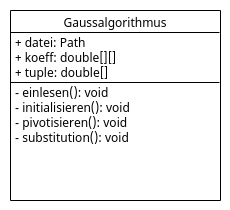
\includegraphics[width=150px]{"./gaussuml.png"}
    \caption{Implementationsdiagramm der Klasse Gauß-Algorithmus}
\end{figure}
\newline
Die Methode einlesen() liest die Koeffizienten einer Matrix aus einer txt-Datei ein, dabei filtert sie jegliche Kommentare
sowie Leerzeichen aus dieser heraus, und speichert die Koeffizienten in dem Array koeff[][].
Die ausgabe() gibt sowohl die Eingangsmatrix, als auch die Lösungsmatrix auf der Konsole aus, indem über die beiden Arrays koeff[][] und mx[][] iteriert wird
und ihre Indizes ausgegeben werden.
Die Methode multiplyandadd() manipuliert die Zeilen der Eingangsmatrix, indem sie die Zeilen dieser
mit dem Faktor multipliziert, der benötigt wird, um bei der Addition mit der nächsten Zeile eine Null herzustellen. Durch die Forschleife wird jede Spalte der angegeben
Zeile durchlaufen und der Parameter linetwo aktualisiert.
Die Methode copyline() kopiert die Eingangsmatrix in eine Hilfsmatrix, damit die Eingangsmatrix erhalten bleibt und am Ende ausgeben werden kann.
Die Methode gaussAlgo() ist das Herzstück des Programms.i %Hier muss die Erläuterung des fertigen Algorithmus erfolgen!!!%


\section{Beispiel Rechnungen}
\chapter{Abwägungen}

\section{Vorteile des Algorithmus}
Der Gauß-Algorithmus hat klar den Vorteil das er bei Gleichungssystemen mit wenig Koeffizienten sehr effektiv ist, d.h er kann die Lösung schnell und einfach berechnen.
Auch ist der Algorithmus in der Programmierung relativ leicht umzusetzen, da er nach einfachen Schemata funktioniert, es werden wenig Schritte benötigt.
Ein weiterer Vorteil ist, dass der Algorithmus auch erweitert werden kann um beispielsweise invertierte Matrizen und/oder Eigenwerte und Eigenvektoren von Matrizen zu berechnen.
\section{Nachteile des Algorithmus}
Zum einen kann es durch die Verwendung vom Datentyp Double und die mehrfache Rechnung mit denselben Werten zu Rundungsfehlern kommen.
Zum anderen hat der Algorithmus bei komplizierten Martizen mit vielen Zeilen und Spalten eine große Laufzeit, die Worstcase Laufzeit würde aufgrund von doppelten for-Schleifen $ O(n x n) $ betragen.
Nachteile des Algorithmus sind zum einen, dass bei schlecht konditionierten Gleichungssystemen Rundungsfehler auftreten können.
Dies sieht man auch in der vorliegenden Implementation, wobei durch die Verwendung vom Datentyp double und dem rechnen mit denselben gerundeten Zahlen noch größere Rundungsfehler entstehen können.
Außerdem kann der Algorithmus bei vielen Koeffizienten eine
sehr hohe Rechenleistung in Anspruch nehmen.
\chapter{Anwendungsbereiche des Gaußschen-Eliminationsverfahrens in der Informatik}
Der Algorithmus spielt in der Informatik aufgrund seiner Simplizität eine tragende Rolle in vielen Teilbereichen, wie der Kryptografie, der Computergrafik oder der Datenanalyse. Die Anwendungsmöglichkeiten, in diesen werden im Folgenden erläutert.
\section{Kryptografie}
Das Gauß'sche Eliminationsverfahren kann verwendet werden, um modulare Gleichungen zu lösen, die in der Kryptografie häufig auftreten.
Zum Beispiel wird das Verfahren bei der Berechnung von Schlüsseln in asymmetrischen Kryptosystemen wie RSA eingesetzt. Hierbei wird mit dem Gaußalgorithmus eine Primfaktorzerlegung durchgeführt, die dann
verwendet, um Schlüssel in asymmetrischen Kryptosystemen zu verwenden. Mehr Informationen in \cite{3} Kapitel 11.4.3.

\section{Computergrafik}
In der 3D-Computergrafik werden 4x4-Matrizen verwendet, um Objekte im Raum zu transformieren.
Diese Matrizen enthalten Informationen über Translationen, Rotationen und Skalierungen von Objekten.
Das Gauß'sche Eliminationsverfahren wird verwendet, um die inverse Matrix zu berechnen, die dann verwendet wird,
um die Transformationsoperationen umzukehren. Die inverse Matrix wird auch dazu verwendet, um Normale von 3D-Objekten zu transformieren,
um sie in eine konsistente Richtung zu bringen, was wichtig ist für Beleuchtungs- und Schattierungsberechnungen.

\section{Datenanalyse}
Das Gauss'sche Eliminationsverfahren wird in der linearen Regression eingesetzt, um die beste Anpassung einer linearen Funktion an gegebene Daten
zu finden. Es wird verwendet, um die Parameter der Funktion zu berechnen, die am besten zu den Daten passen, indem es die Summe der Quadrate der Fehler minimiert. Die lineare Regression ist ein wichtiges Werkzeug in der Datenanalyse, um Beziehungen zwischen Variablen zu identifizieren und Vorhersagen über zukünftige Daten zu treffen.
Das Verfahren kann auch dazu verwendet werden, um die Koeffizienten eines linearen Gleichungssystems zu lösen, das in der Datenanalyse oder der Signalverarbeitung verwendet wird.
\chapter{Fazit}
\chapter{Anhang}
\lstinputlisting[language=Java, caption=Quellcode des Gauß-Algorithmus]{./Quellcode/Gauss.java}
\printbibliography
\end{sloppypar}
\end{document}
